\section{Initial Optimization}
This section describes the initial optimization on the simplified problem with two variables. All other variables were set to constant values in the feasible domain. 
\subsection{Straight Design}
Two variables: $w_b$ and $F$ were optimized to investigate the implementation of the SQP algorithm. The other variables, $h_f$, $v_a$ and $v_b$ were set to 1.0, 2.0 and 1.0 respectively such that these lie inside the feasible domain. The starting point was set to $[w_b F] = [1, 1]$ and the SQP algorithm was executed. The result is shown in \autoref{fig:straightopt}. As can be seen, the algorithm converges along constraint $g_{ca}$ towards the optimum of $[w_b F] = [2.25 23.56]$ mm, N. The minimized value of the objective function is then 0.145 mm$^2$/N, thus the maximum strength equals 6.90 N/mm$^2$ for this configuration. Constraints $g_{ca}$ and $g_{tb}$ are active. It takes 152 iterations till convergence.


\begin{figure}[H]
	\centering
	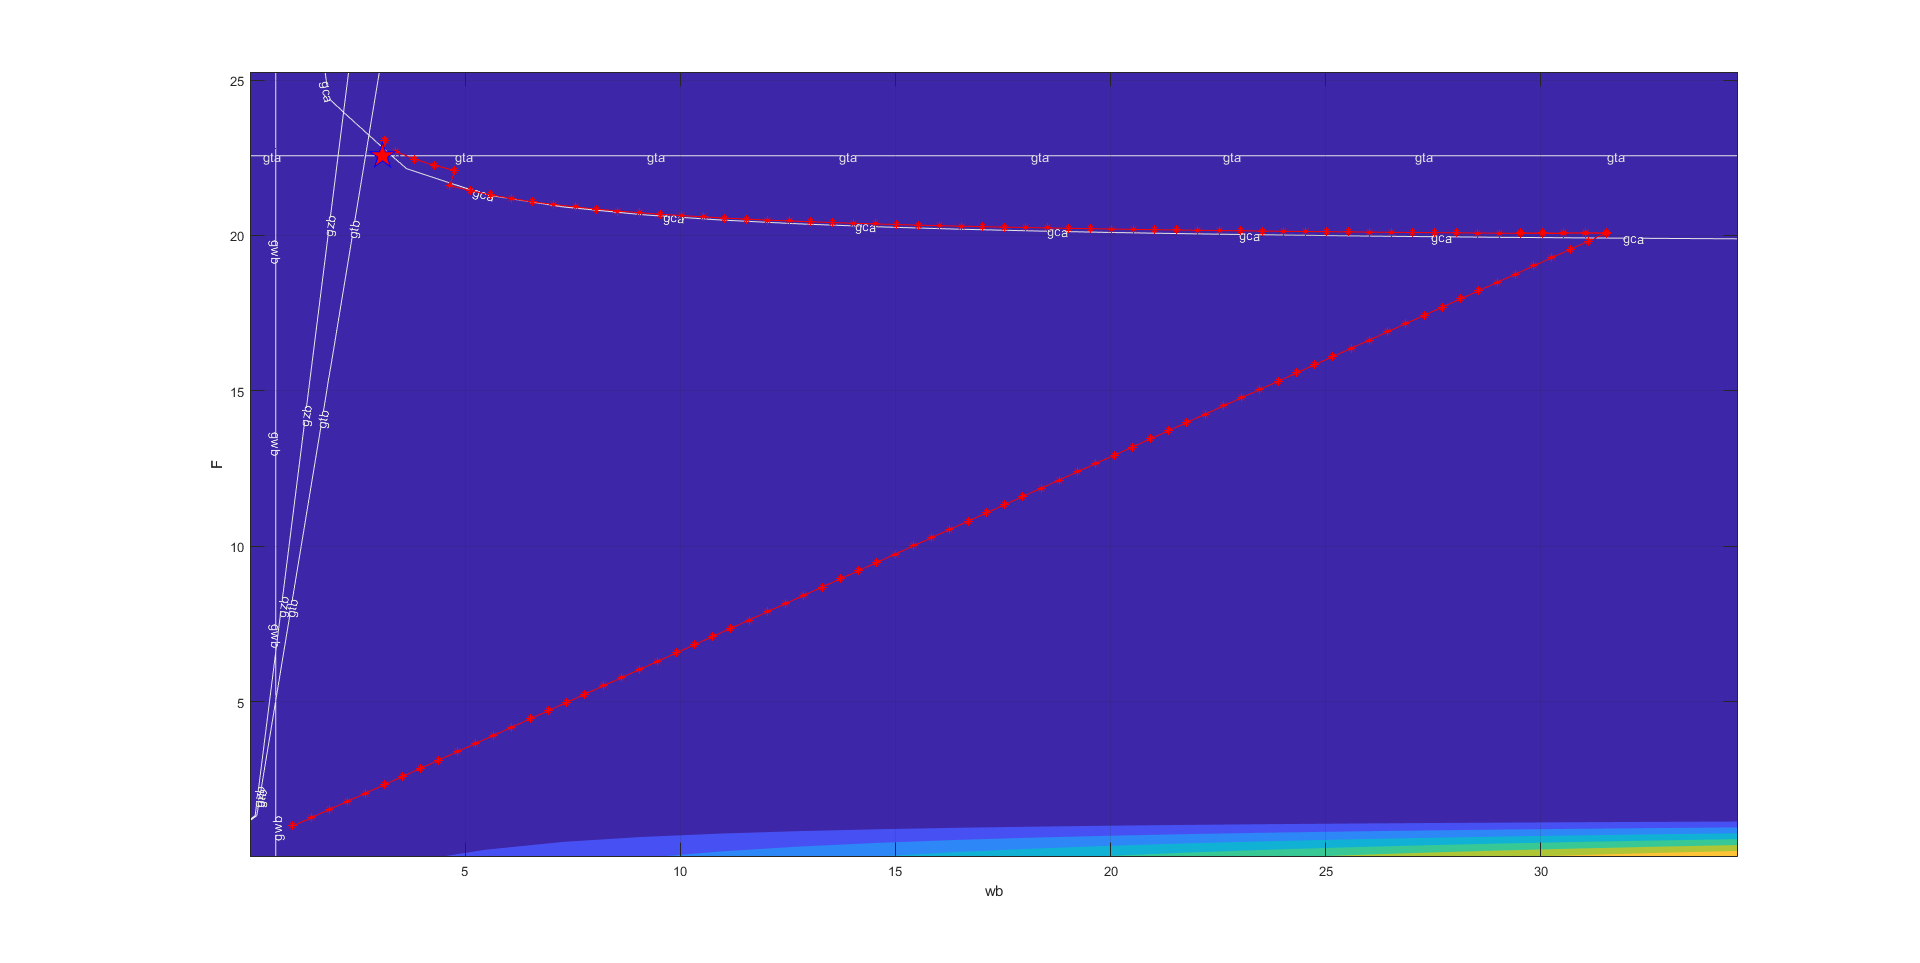
\includegraphics[width=\columnwidth]{sources/plots/straight2var.png}
	\caption{The optimization steps taken by the SQP algorithm for the design variables $w_b$ and $F$ in the straight design.}
	\label{fig:straightopt}
\end{figure}


\subsection{Diagonal Design}
The same SQP algorithm was also tested on the diagonal design. Again, $w_b$ and $F$ were optimized with an initial value of $[w_b F] = [1, 1]$. The other design variables $w_a$ and $L$ were set to 1.0 and 3.0 respectively. \autoref{fig:diagopt} shows the result, where $w_b$ and $F$ converge to 2.36 mm and 4.59 N respectively. This gives a minimized objective of 0.732 mm$^2$/N, equal to a maximum strength of 1.37 N/mm$^2$.


\begin{figure}[H]
	\centering
	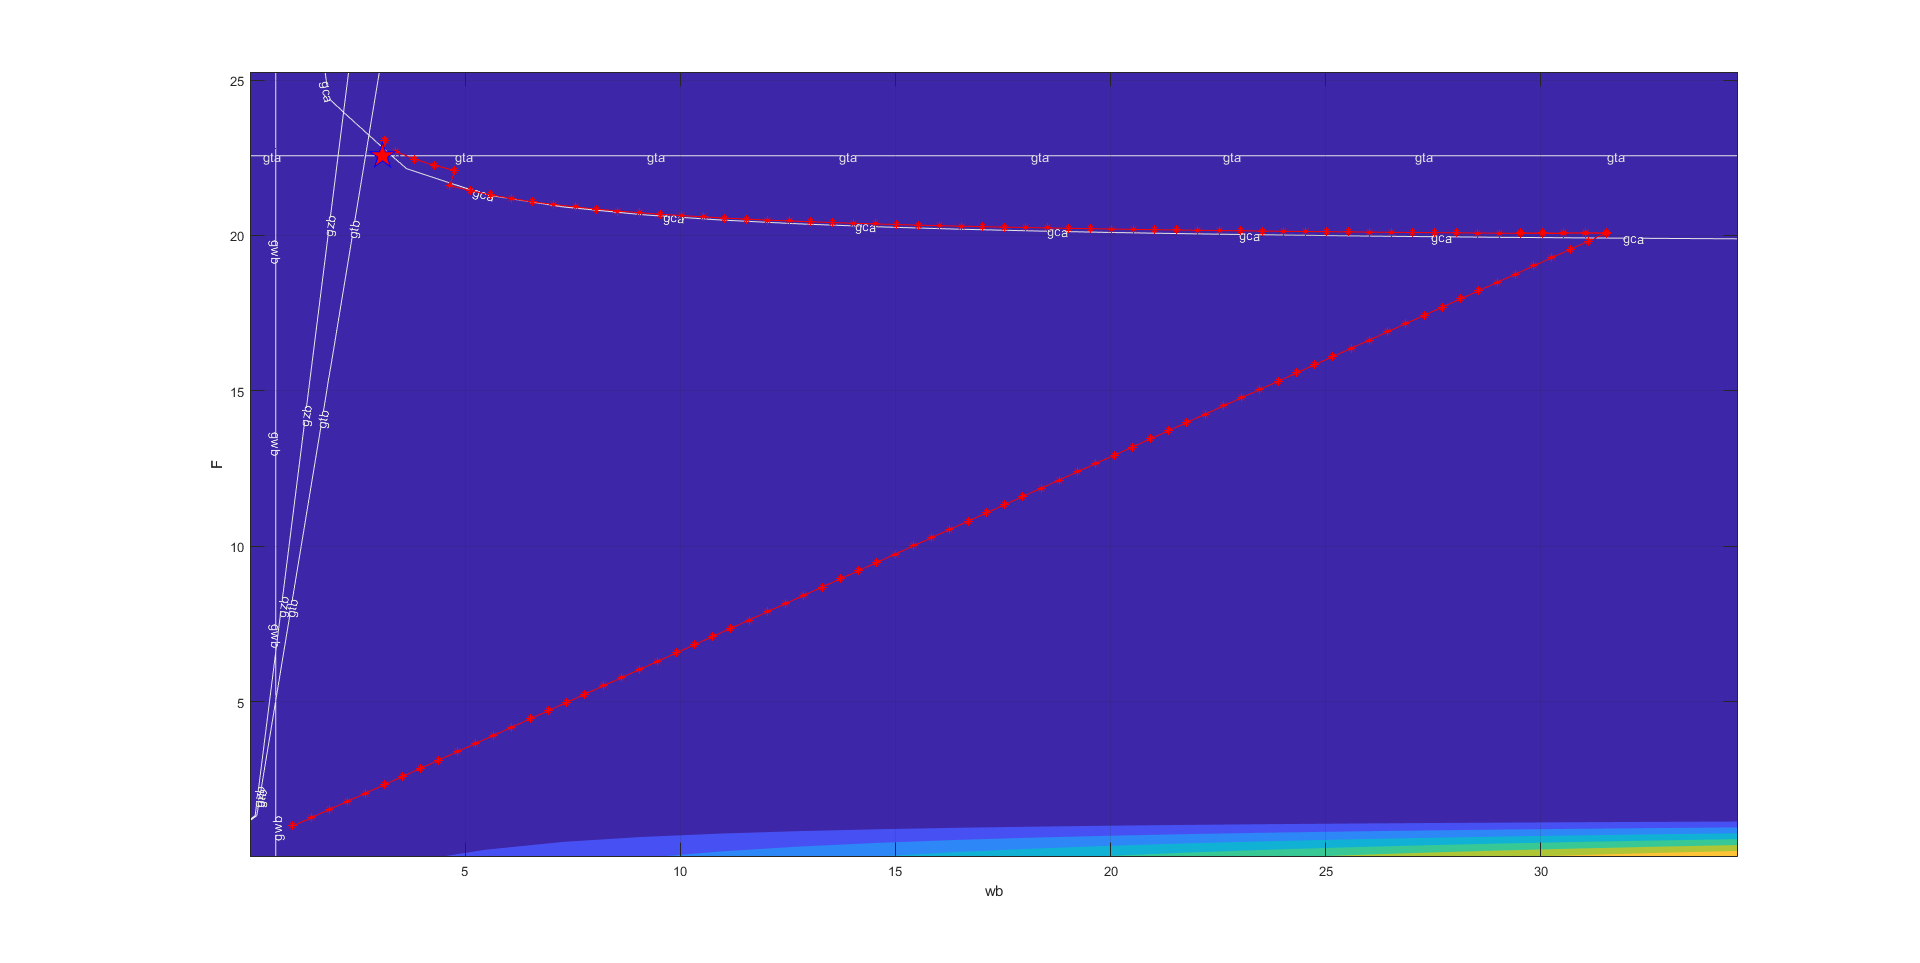
\includegraphics[width=\columnwidth]{sources/plots/straight2var.png}
	\caption{The optimization steps taken by the SQP algorithm for the design variables $w_b$ and $F$ in the diagonal design.}
	\label{fig:diagopt}
\end{figure}








